%%%%%%%%%%%%%%%%%%%%%%%%%%%%%%%%%%%%%%%%%
% Masters/Doctoral Thesis 
% LaTeX Template
% Version 1.43 (17/5/14)
%
% This template has been downloaded from:
% http://www.LaTeXTemplates.com
%
% Original authors:
% Steven Gunn 
% http://users.ecs.soton.ac.uk/srg/softwaretools/document/templates/
% and
% Sunil Patel
% http://www.sunilpatel.co.uk/thesis-template/
%
% License:
% CC BY-NC-SA 3.0 (http://creativecommons.org/licenses/by-nc-sa/3.0/)
%
% Note:
% Make sure to edit document variables in the Thesis.cls file
%
%%%%%%%%%%%%%%%%%%%%%%%%%%%%%%%%%%%%%%%%%

%----------------------------------------------------------------------------------------
%	PACKAGES AND OTHER DOCUMENT CONFIGURATIONS
%----------------------------------------------------------------------------------------

\documentclass[11pt, oneside]{Thesis} % The default font size and one-sided printing (no margin offsets)

\graphicspath{{Pictures/}} % Specifies the directory where pictures are stored

\usepackage[square, numbers, comma, sort&compress]{natbib} % Use the natbib reference package - read up on this to edit the reference style; if you want text (e.g. Smith et al., 2012) for the in-text references (instead of numbers), remove 'numbers' 
\usepackage[english]{babel}

\hypersetup{urlcolor=black, colorlinks=true} % Colors hyperlinks in blue - change to black if annoying
\title{\ttitle} % Defines the thesis title - don't touch this

\usepackage{listings}
 \usepackage{courier}


\begin{document}

\frontmatter % Use roman page numbering style (i, ii, iii, iv...) for the pre-content pages

\setstretch{1.3} % Line spacing of 1.3

% Define the page headers using the FancyHdr package and set up for one-sided printing
\fancyhead{} % Clears all page headers and footers
\rhead{\thepage} % Sets the right side header to show the page number
\lhead{} % Clears the left side page header

\pagestyle{fancy} % Finally, use the "fancy" page style to implement the FancyHdr headers

\newcommand{\HRule}{\rule{\linewidth}{0.3mm}} % New command to make the lines in the title page

% PDF meta-data
\hypersetup{pdftitle={\ttitle}}
\hypersetup{pdfsubject=\subjectname}
\hypersetup{pdfauthor=\authornames}
\hypersetup{pdfkeywords=\keywordnames}

%----------------------------------------------------------------------------------------
%	TITLE PAGE
%----------------------------------------------------------------------------------------

\begin{titlepage}
\begin{center}
\begin{figure}[htbp]
\begin{center}

\includegraphics[width=4cm]{Figures/logo.png}
\end{center}
\end{figure}

\textsc{\LARGE \univname}\\[1.0cm] % University name
\textsc{\Large Diploma Accademico Ordinamentale di I livello}\\[0.3cm] % Thesis type

\HRule \\[0.4cm] % Horizontal line
{\huge \bfseries \ttitle}\\[0.5cm] % Thesis title
\HRule \\[0.4cm] % Horizontal line
 
\begin{minipage}{0.4\textwidth}
\begin{flushleft} \large
\emph{Author:}\\
\href{http://www.johnsmith.com}{\authornames} % Author name - remove the \href bracket to remove the link
\end{flushleft}
\end{minipage}
\begin{minipage}{0.4\textwidth}
\begin{flushright} \large
\emph{Supervisor:} \\
\href{http://www.jamessmith.com}{\supname} % Supervisor name - remove the \href bracket to remove the link  
\end{flushright}
\end{minipage}\\[2cm]
 
\large \textit{A thesis submitted in fulfilment of the requirements\\ for the degree of Bachelor}\\[0.6cm] % University requirement text

\groupname\\\deptname\\[2cm] % Research group name and department name
 
%{\large \today}\\[4cm] % Date
%\includegraphics{Logo} % University/department logo - uncomment to place it
\large Anno Accademico 2013/2014 \\ Sessione terza
 
\vfill
\end{center}

\end{titlepage}


%----------------------------------------------------------------------------------------
%	QUOTATION PAGE
%----------------------------------------------------------------------------------------

\pagestyle{empty} % No headers or footers for the following pages
\null\vfill\vfill\vfill
\begin{flushright}
\emph{Itaca tieni sempre nella mente.\\
La tua sorte ti segna quell'approdo.\\
Ma non precipitare il tuo viaggio.\\
Meglio che duri molti anni, che vecchio\\
tu finalmente attracchi all'isoletta,\\
ricco di quanto guadagnasti in via,\\
senza aspettare che ti dia ricchezze.}
\end{flushright}
\begin{flushright}
\emph{Itaca t'ha donato il bel viaggio.\\
Senza di lei non ti mettevi pi\`u in via.\\
Nulla ha da darti pi\`u.}
\end{flushright}

\null\vfill % Add some space to move the quote down the page a bit


\begin{flushright}
Kostantinos Kavafis,

\emph{Itaca}
\end{flushright}

\vfill\vfill\vfill\vfill\vfill\vfill\null % Add some space at the bottom to position the quote just right

\clearpage % Start a new page

%----------------------------------------------------------------------------------------
%	ABSTRACT PAGE
%----------------------------------------------------------------------------------------

\addtotoc{Abstract} % Add the "Abstract" page entry to the Contents

\abstract{\addtocontents{toc}{\vspace{1em}} % Add a gap in the Contents, for aesthetics

The pitch organisation through time is called \emph{harmony} for polyphonic sounds. The pitch of harmonic sounds can be shifted, that is transposing the note and its height. Harmonising a sound means mixing this with several pitch-shifted version of it to obtain specific chords. Pitch shifting consists in scaling the frequency axis of a time-frequency representation of the sound. When a harmoniser is based on several pitch shifter engines, any of this controlled by the input pitch and the harmonic context, it's called \emph{smart} harmony or \emph{intelligent} harmonisation. To achieve this kind of audio effects, an algorithm for pitch estimation is needed.
}

\clearpage % Start a new page

%----------------------------------------------------------------------------------------
%	ACKNOWLEDGEMENTS
%----------------------------------------------------------------------------------------

\setstretch{1.3} % Reset the line-spacing to 1.3 for body text (if it has changed)

\acknowledgements{\addtocontents{toc}{\vspace{1em}} % Add a gap in the Contents, for aesthetics
This work was written over a period of some months. This is the first time I attempt on a project of such a complexity. Many of the concepts and the subjects of this work were completely new to me. I learned to write in a programming language as C++, learned to use several softwares. I started thinking in a more logical way and that will help me in non-musical fields. Undoubtedly, it has been an educational path rather than a final project. It's a starting point for what I'm to going to do in the future, or for what I would like to do. I hope for possible collaborations that will help me to continue in this research and will allow a more precise and deeper knowledge of what is necessary to this project.

I am profoundly indebted to many generous people for their numerous suggestions. First, my Supervisor Carmine-Emanuele Cella, for his precious time, and big effort. He made me widen my mind, and see the unknown. I'll keep all his influences for years. I would like to thank Lorenzo Pagliei, my main teacher at GRAIM, for his dedication to the Bachelor course. I'd like to thank Davide Tiso for every tip and for the ambition and perseverance I learned from him. I'd also like to thank my classmates: they made our class a very comfortable place where I spent some of the best moments of these past years. I should thank Marzia, who read all this draft and carefully gave me some suggestions to improve the language. I'd like to thank all my professors, and all the people who walked along with me during this time for their patience, comprehension and love, in particular Alessia and my brothers InSpiral. But above all, I should thank my family for giving me the freedom to lead my life.
}
\clearpage % Start a new page

%----------------------------------------------------------------------------------------
%	LIST OF CONTENTS/FIGURES/TABLES PAGES
%----------------------------------------------------------------------------------------

\pagestyle{fancy} % The page style headers have been "empty" all this time, now use the "fancy" headers as defined before to bring them back

\lhead{\emph{Contents}} % Set the left side page header to "Contents"
\tableofcontents % Write out the Table of Contents

\lhead{\emph{List of Figures}} % Set the left side page header to "List of Figures"
\listoffigures % Write out the List of Figures

\lhead{\emph{List of Tables}} % Set the left side page header to "List of Tables"
\listoftables % Write out the List of Tables

%----------------------------------------------------------------------------------------
%	DEDICATION
%----------------------------------------------------------------------------------------

\setstretch{1.3} % Return the line spacing back to 1.3

\pagestyle{empty} % Page style needs to be empty for this page

\dedicatory{For Emily, whenever I may find her\par
\footnotesize Simon \& Garfunkel} % Dedication text

\addtocontents{toc}{\vspace{2em}} % Add a gap in the Contents, for aesthetics

%----------------------------------------------------------------------------------------
%	THESIS CONTENT - CHAPTERS
%----------------------------------------------------------------------------------------

\mainmatter % Begin numeric (1,2,3...) page numbering

\pagestyle{fancy} % Return the page headers back to the "fancy" style

% Include the chapters of the thesis as separate files from the Chapters folder
% Uncomment the lines as you write the chapters

\input{Chapters/Chapter1}
% Chapter 1

\chapter{Algorithm design} % Main chapter title

\label{Chapter2} % For referencing the chapter elsewhere, use \ref{Chapter1} 

\lhead{Chapter 2. \emph{Algorithm design}} % This is for the header on each page - perhaps a shortened title

%----------------------------------------------------------------------------------------

The aim of this chapter is to give the reader the most important information about the algorithms used in this work, their implementation and their specific differences relative to what has been already said in \ref{Chapter1}.

Research has been conducted this way: first of all, it has been examined all the literature about a specific technique; then, an own implementation has been done in C++. So it has been produced two main codes: one for the pitch detection, the other for the pitch shifting. These codes, specifically, represent the engines of the relative MSP externals presented here. Before introducing these codes within the tools provided by \emph{Max SDK} (the Cycling 74's Software Developer Kit) in order to build these externals, a command-line version of the codes is made, so to test and improve them easily. Finally, Xcode 6 has been used to realise an \textbf{.mxo} object that will be recalled inside the Max 6 patcher built by the Author and the Supervisor together.
\clearpage

\section{Fundamental decisions}
%perch� algoritmo AMDF e non altro?
%perch� median filter?
An AMDF-based algorithm for pitch estimation has been chosen because it better suits to the requests of the Intelligent Harmonizer, that are working in real-time and with a small computation cost. In order to prevent and eliminate the problems involved with the use of this technique, several improvements are proposed inside the algorithm. Moreover, it's been added a \emph{median-filter} section after the pitch detection stage to smooth undesired and too fast frequency changes due to the limits of this technique and to the possible issues of the signal. 

%perch� algoritmo pitch shift?
To achieve pitch transposition, delay-lines based pitch shifter sums up a certain simplicity in the implementation of its code, together with a low cpu amount and a good sound quality - it doesn't require many improvements. Furthermore this approach allows to process the sound without switching to frequency-based domain, as it's the case of the phase vocoder instead. 

\section{Implementation}
\subsection{Pitchdetect$\sim$}
\label{pitch}
First, the input signal is passed through a low pass filter to improve the accuracy of this technique \cite{rabiner1976comparative} (and also to cut off a part of the spectrum not useful for the pitch estimation). Then the AMDF algorithm takes place, as shown in the following listing:
\newline
\begin{lstlisting}
for (int n = 0; n < N2; ++n) {
		float diff = 0;
		rms += (buffer[n] * buffer[n]);
		for (int m = 0; m < N2; ++m) {
			diff += fabs (buffer[m] - buffer[m + n]);
		}
		diff *= pow (n, coeff);
		amdf[n] = diff;
		if (maxAmdf < diff) maxAmdf = diff;
	}
	
\end{lstlisting}

%1. modifiche all'algoritmo classico
We might observe an important revision of the classic algorithm implementation shown in \cite{ross1974average, ying1994probabilistic, zhao2013amdf, muhammad2008noise}. Unlike traditional AMDF, this version computes two independent loops, one internal to the other. These loops count from zero to half buffer. So, herein, we could suppose the range in which the difference is calculated, isn't the whole buffer length. Despite this supposition, all the buffer samples are taken into account to compute the minimum difference. In fact, while the external loop increases the value of $n$, the internal one increases $m$. So, for instance, when $n = N2 - 1$ (e.g. half buffer) the range of $[m + n]$ varies from $N2 - 1$ to $N - 1$. We have \emph{in any case} a full comparison within the buffer. This strategy shorten the time in which the computation is done, allowing for better real-time performance without wasting cpu resources.

%2. scelta di treshold, bias e confidence
\textbf {Threshold and Bias.}
We might notice a specific parameter in the listing above: \emph{coeff}. What does it mean? It has been previously said that AMDF technique suffers from possible falling tendency \cite{muhammad2008noise}. This explains why sometimes the frequency estimated is lower, compared to the expected one. One possible solution is to partially modify the result of summation by well averaging the lag values. In this work, \emph{coeff} means how much the values are averaged. Because \emph{coeff} is the exponent, its right values shouldn't be less than 1. For coeff = 1, the difference value remains the same calculated by AMDF. If we increase this value, we raise the difference value and, obviously, the entire summation. 
This parameter, inside the external structure, is called \emph{bias}.
\newline
\begin{lstlisting}
int minLag = (1. / maxF0) * sr;
	int maxLag = (1. / minF0) * sr;

	if (rms < threshold) return 0;
\end{lstlisting}

As shown in the listing above, the parameter \emph{threshold} defines when the input signal has to be considered as silence or as sound. The higher the threshold value, the less the estimated values that pitchdetect$\sim$ outputs. In fact, at the same time pitch detection is done, the algorithm also computes the RMS (\emph{root mean square}, that is the energy of the signal) on the entire buffer. If this RMS value is less than the threshold one, supposed the energy value is given in linear amplitude, the system will output a zero value: no fundamental frequency is given because there's no harmonic sound in the signal.

\textbf{The absolute minimum.}
First of all, the research of the minimum difference is limited inside a specific range, whose side values are given by the user. These are called \emph{min} and \emph{max frequency}. The user should keep in mind that this algorithm, as almost every detection algorithm, could exhibit some issue at its extreme values, so to select an accurate range. For instance, a more precise detection of a 100 Hz fundamental could't be made if the \emph{min frequency} parameter is set to the same value. 
\clearpage
\begin{lstlisting}
for (int i = minLag + 1; i < maxLag - 1; ++i) { //safety
		if (amdf[i] < amdf[i - 1] && amdf[i] < amdf[i + 1]) {
			minimaPos[currentMinimum] = i;
			minima[currentMinimum] = amdf[i];
			++currentMinimum;
 		} 
	}  
\end{lstlisting}

In this stage of the research, every AMDF value previously calculated (whose index is in the range determined by the user) is compared with the one before and the one after. If this value is the lowest, then we have a local minimum. Its value and its position (i.e. the samples at which we have the minimum) are stored. 
\newline
\begin{lstlisting}
	for (unsigned int i = 0; i < currentMinimum; ++i) {
		if (minima[i] < min) {
			min = minima[i];
			index = i; 
		}
	}
\end{lstlisting}

Next, all the local minimum are compared each other to get the absolute minimum and, in particular, its sample position. In fact, the \emph{index} found refers to the array of indexes \emph{minimaPos}. The value that pitchdetect$\sim$ outputs is $sr / minimaPos[index]$, where \emph{sr} is the sampling rate - that is, a value in Hertz that corresponds to the fundamental frequency for the examined buffer of input signal.


\subsection{Dlshift$\sim$}
\label{dlshift}
%1. descrizione e references
Dlshift stands for \emph{delay-line} shifting.
This approach leads to a quite simple implementation and requires no large CPU resources to let a multiple utilisation possible.

%pitch shifting tramite phasor~
\textbf{Circular buffers.}
Generally speaking, the pitcher effect is created by increasing or decreasing the delay by a fixed amount \cite{lazzarini2010audio}. If looked from a different view, we could think of it as a circular delay line constantly re-written, as it was a wavetable. The term \emph{circular} means that the reading and the writing point of the the delay line are dynamics, changing their position along the line itself. This allows to keep the length of the buffer quite short in order to let the user not to perceive a significant delay of the processed sound relative to the original one. This leads to an important consideration: there always will be a little amount of delayed signal that gives the Harmonizer the classic \emph{phasing} effect \cite{zolder2011dafx}.

The delay reading point then proceeds through the line with an increment that reflects the desired pitch transposition rate. If its position increment is 1, there's no pitch transposition - and then, no delay change. If the increment is major than 1, we're playing the delay line at a faster rate than the rate at which it was written, so to have an upward transposition. Conversely, if the increment is between 0 and 1 the pitch is shifted downward.   

\textbf{Main features.}
In this implementation, pitch shifting is achieved using two time-varying delay lines. The continue modulation is provided by a sawtooth-type function \cite{zolder2011dafx}. For its similarity to the relative MSP object, this is called \emph{phasor} to remind the principle on what the \emph{phasor$\sim$} is based, that is to generate a sawtooth function expressed in Hz. So, it's required to allocate externally a one-second length buffer to write a sawtooth function in. The length of this buffer depends on the sampling rate of the system. The rate at which the sawtooth function is played is given by the different increment of the reading index of the table. One of the parameters the user is asked to input at the MSP external initialisation, \emph{phasor frequency}, is exactly how much the reading index has to move forward every loop step in order to achieve the desired transposition rate.

Here is the central point of shifter code.
\newline
\begin{lstlisting}
out = (frac * D1[next] + (1.0 - frac) * D1[rpi]) * x; 
		out += ((frac2 * D2[next2] + 
			(1.0 - frac2) * D2[rpi2])) * (1 - x);
		D1[(int)wptr] = sig[n];
		D2[(int)wptr] = sig[n];
		outbuffer[n] = out;
		
		++wptr;
		wptr %= dt;
        	tablePos += (pf);
        	if(tablePos < 0.) tablePos += len;
        	if (tablePos >= len) tablePos -= len;
\end{lstlisting}

This is included in a main loop that also contains the calculation of \emph{phasor}, \emph{cosine} and \emph{reading point} values. The conditions of this loop are: for $n = 0; n < N; ++n$, where $N$ is the vector size length. We might notice how the algorithm works doing these actions in the following order \cite{lazzarini2010audio}: 
\begin{enumerate}
\item both the delay lines are read at their current reading position and summed up together to generate the output;
\item the input signal is written that position on every buffer;
\item the reading positions are incremented.
\end{enumerate}

In particular, the algorithm always checks if the reading point has reached the end of the delay line. In fact, we should keep in mind that the vector size is generally smaller than the delay line - this time, we choose a 50 ms long delay line. It needs the writing position index to be saved before a new buffer of audio signal comes in, so to resume the count during the successive loop. To do that, we pass to the function a \emph{reference} value, and so does for the reading position index of the phasor table. In other words, we are passing the variable itself and not a copy of it and the last value is always kept inside the memory location until it's cleared. Then, the modulus operation guarantees that the variable \emph{wptr} never overcomes the maximum value of delay time (\emph{dt}).

%interpolazione lineare
\textbf{Linear interpolation.}
Analogous, but slightly different, is the matter of the increment of the phasor table. Here, we could have a non-integer increment due to the fractional \emph{phasor frequency} value. So how to calculate correctly the value from a table that accepts \emph{only integer} indexes?
\newline
\begin{lstlisting}
tableFloor = floor (tablePos);
tableFrac = tablePos - (float) tableFloor;
tableNext = (tableFloor + 1 == len? 0 : tableFloor + 1);
phasor_value = (1. - tableFrac) * table[(int) tableFloor] +
			tableFrac * table[tableNext];
\end{lstlisting}

The answer is the linear interpolation, and its formula is:
\begin{equation}
(1 - frac) \cdot x + frac \cdot (x + 1)
\end{equation}
\newline
Practically, a linear interpolation makes sense only if we consider two integer values at a time. These are the operations requested:
\begin{enumerate}
\item calculate the maximum integer value that is not greater than the fractional one (in this case, we're using the C++ \emph{floor} function);
\item calculate the fractional part of the original value;
\item focus on the integer value next to the one we have already calculated and check if it falls inside the phasor buffer;
\item now, it's possible to do linear interpolation.
\end{enumerate}

All the values involved in linear interpolation let the algorithm calculate the other required variables in the loop: the reading position indexes (through \emph{phasor\_value}) and the cosine value corresponding to the phasor table position.

\section{Issues}
In the following section, the main issues observed during the implementation stage are briefly shown. A possible solution, or a discussion for a future improvements will be provided. Some of this enhancements take their name from similar parameters that Cella's \emph{Revoice} exhibits.

%1. vector size issues and downsampling
\subsection{Vector size issues and \emph{downsampling}}
One of the main problems of both implementations is that they don't have \emph{fixed} vector size values inside. 
This characteristic initially could not represent such a hard problem but changing the vector size from the Max \emph{Audio Setup} window while the algorithm is working can cause undesired clicks, loss of data and, in some cases, it can suddenly stop working.
To fix this, we could think of a buffer independence.
First, we could declare a constant called \emph{internal\_buffer\_size} and give it an average value that best suits any case. For any vector size value selected externally, it could be calculated the algorithm's \emph{downsampling} factor, that is how many buffers the system has to input to completely fill its internal one. Once the internal buffer is filled with signal, the process - whatever it is - can take place.

%2. confidence
\subsection{The \emph{Confidence} parameter}
The pitch detection algorithm described before exhibits, in some critical situation, undesired values that make us not very \emph{confident} about their possible use. In particular, when used with vocals or non-tempered instruments it may be output all the pitch-period fluctuation, resulting in microtonal pitch. That's truly correct, but it may give us some problems in using these non-tonal values, for instance in calculating the interval between this note and a root key note. 

Pitchdetect$\sim$ gives the user a parameter to control these possible undesired values, and this is called \emph{confidence}. In practice, this acts like a pseudo-ratio semitone value. Two separate frequency values are calculated with confidence one, \emph{minpitch} and \emph{maxpitch}. Then, the last detected frequency is compared with these ones. If this value stays between the smaller and the greater, no \emph{tonal} change in pitch happened in the signal. So, the algorithm doesn't output the the last pitch-period but the previous one and so does until the last detected value falls out of this range. All the process is shown in the listing below.
\newline
\begin{lstlisting}
float minpitch = m_oldpitch / m_ratio;
float maxpitch = m_oldpitch * m_ratio;
if ((m_pitch > maxpitch || m_pitch < minpitch) || m_oldpitch == 0) {
	m_oldpitch = m_pitch;
}
\end{lstlisting}

%3. median filter
\subsection{Using a \emph{median filter}}
In order to prevent too fast pitch-period changes, not useful if we're using them in tracking some else musical parameter, pitchdetect$\sim$ has been provided with a median filter to smooth the output values curve. It's more likely we're interesting in a well-balanced pitch estimation through audible time segments rather than a more precise estimation at every vector size. Generally speaking, the more a parameter is recognised to belong to the human sphere, the more impressive its musical result will be.
\newline
\begin{lstlisting}
for (int i = 0; i < MEDIANSIZE; ++i){
                m_median[i] = m_amdf_tmp[i];
}
bsort (m_median, MEDIANSIZE);
m_pitch = m_median[MEDIANSIZE / 2];
\end{lstlisting}

Typically used on signals that may contain outliers skewing the values we're waiting for, a median filter takes a list of $N$ values, sorts this in an increasing order and, finally, returns the middle value \cite{devillard1998fast}. From that, a median filter allows a smoother distribution. The only cost is a delay of $N$ vector sizes before it returns the first real value. In fact, it has to wait that all the array designated to be filtered is filled to obtain the first significant value. Moreover, as shown in the listing above, we should create a \emph{copy} of this array to let the pitch output order not be altered from sort operation. The length of this array is chosen out of the algorithm and generally is an odd number.

%4. de-clicking in pitch shifter?
\subsection{De-clicking and modulation in pitch shifting}
\label{delissue}
We said that the delay line is finite and circular. So, at some point, either the reading point will overtake the writing point or vice versa \cite{lazzarini2010audio}. This may happen because the reading tap is moving with a different increment than the writing one, that is the reading taps is moving through the buffer at its own rate. This will create audible popping sounds and a nasty click in the signal when the sawtooth comes back from its end to its beginning. The best way to avoid the click is to add an envelope (sometimes called a \emph{window}) that goes to zero at that discontinuity. This can be, as it is in the case of this work, a cosine shape, going from 0 at its end to 1 in the middle. 

However, the signal is now de-clicked but with an important modulation. The sound periodically disappears when the envelope goes to zero. In order to reduce this \emph{tremolo-like} effect, which is generally undesirable, we can use a second reading point (or, better, a second delay line with its own reading point) that is offset by half a delay length, and enveloped in the same way. So, when one tap is at its discontinuity point (and thus its amplitude is zero), the other tap is at its maximum amplitude. This results in a smoother output, with no click and less disturbing amplitude modulation. The cosine shape curve fits naturally any possible amplitude fluctuation due to the \emph{crossover} stage. This methods comes from the old 2-tap pitch shifter implementation in devices like Eventide H910 and H949. The use of several reading taps, or several delay lines, is perceived as a phasing-like effect artifact that is less annoying anyway \cite{zolder2011dafx}.  



\section{Conclusion}
This chapter has provided a detailed presentation of both the MSP externals built in this work. The main features of pitch detection stage and pitch shifting process have been explained. Later, it has been presented several issues that the Author and the Supervisor have passed through. In particular, we focused on possible issues that AMDF algorithms can exhibit when performing on complex material (i.e. speech or very noisy signal). In those cases, pitch-period values could be wrong or different to what we expected. Moreover, we said that the quality of pitch shifting sound can be altered by some undesired sounds, as periodic clicks. At the present time, our pitch shifting implementation is still presenting some artifacts due to possible errors in algorithm implementation. Surely, its sound quality could be improved using a frequency domain technique, as the phase vocoder \cite{laroche1999new}.
Many of the issues described herein have been fixed, others will be surely dealt with in a future.







 
% Chapter 3

\chapter{Use cases and performance} % Main chapter title

\label{Chapter3} % For referencing the chapter elsewhere, use \ref{Chapter1} 

\lhead{Chapter 3. \emph{Use cases and performance}} % This is for the header on each page - perhaps a shortened title

%----------------------------------------------------------------------------------------
%summarize briefly:
%1. patcher presentation
In this chapter, a more specific description about the device's programming stage is given. During this, it has been chosen Cycling 74's \textbf{Max 7} as programming software for its best suitability for the Author and the Supervisor's ideas. 
%2. instrument aim
The principal aim on which all the work is based is to provide the user a device that feeds his musical character and ideas. We focused on the ideas of an \emph{effortless} use and a \emph{musical} one. The user neither should care about programming or technical aspects, nor it's required him some practical knowledge about audio effects. 
Obviously, such a complex device requires some experience. We have tried to overcome this trouble giving the user all the device controls in a nutshell. There are many selection menus, clear parameter visualisation and gain meter for monitoring the input and output signal amplitude. Finally, the user interface is given with a plain harmonisation section: two staves take place. In the former, the estimated pitch of the incoming signal is shown. In the latter, the chord built on the selected harmonisation is shown. 
\clearpage

\section{Musical Aspects}
\label{musical}
%1. harmonic function recognition
\subsection{Harmonic context recognition}
\label{recognize}
As said earlier in the abstract, an \emph{intelligent} harmonizer should take into account not only the pitch-period of the incoming signal, but also the harmonic function at a specific moment. In practice, it should know which degree scale every note is and give it the right harmonisation. This means that there are two main parameters the user had to select previously in order to let the harmonizer work correctly: the \textbf{root key} and the \textbf{scale mode} (see Figure \ref{harm-param}).

The first, \emph{root key}, is a sort of master key that informs the harmonizer about the \emph{tonality} in which the incoming signal is playing (e.g. a musician singing a piece of melody in B). So, for every estimated pitch-period the device calculates its relative degree, expressed in pitch. For instance, if the estimated frequency is the fundamental its pitch degree is 0, if it's the dominant its pitch will be 7, and so on. 

The concept comes from the \emph{pitch set class} theory. For simplifying melodic or harmonic models in atonal music, a new classification was presented in early XX century. In this model, the octave is divided into 12 semitones, as the tempered system, but each semitone is named with a number that ranges from 0 to 11. This model easily fits our purpose because it allows us to make \emph{absolute} chords configuration - in fact, for convenience 0 is always $C$, if not specified any other note.
\begin{figure}[htbp]
\begin{center}
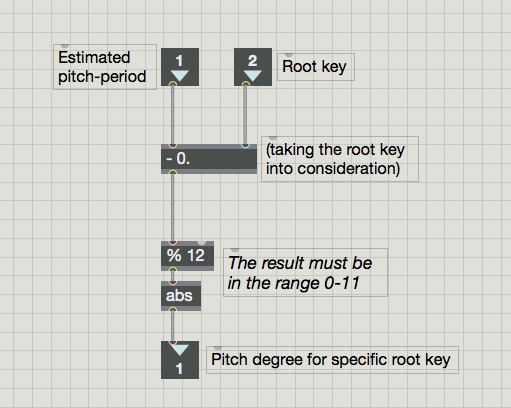
\includegraphics[width=7cm]{Figures/inoctave.png}
\caption{The \emph{inoctave} Max external.}
\label{inoctave}
\end{center}
\end{figure}
\newline
As shown in Figure \ref{inoctave}, we \emph{must} take into consideration the selected root key in order to achieve the right degree value. We have already said that pitch value is \emph{absolute}, i.e. tonality is not considered, and so isn't the octave. We should consider whatever octave and give 0 to the lower considered value, that is the \emph{tonic}. In doing that, we have to convert the root key itself in pitch value and subtract it to the estimated one. For instance, if we have $D$, or 2 in pitch value, and the root key is $C$, its degree value will be 2, the supertonic. On the other hand, if the root key is $D$, we have previously subtracted 2 to the estimated value and so its degree value now is 0, i.e. it's the tonic.
The modulus operator let the result always remain in the established range $0 - 11$, as the pitch class set wants. The value found inside this Max external is the pitch period harmonic function and will be used to select the specific chord the Intelligent Harmonizer will use for this note.

%2. harmonisation control stage
\subsection{Chord selection control stage}
\label{harmonisation}
\begin{figure}[htbp]
\begin{center}
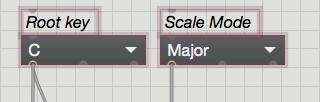
\includegraphics[width=5cm]{Figures/root-key.png}
\caption{\emph{Root key} and \emph{scale mode} parameters.}
\label{harm-param}
\end{center}
\end{figure}
The second parameter shown in Figure \ref{harm-param}, \emph{scale mode}, determines in which manner the harmonisation takes place. Here, the user can switch between different typologies of harmonisation. Each of this has its own musical character, with its own chordal voices displacement:
\begin{itemize}
\item \emph{Major} mode provides a major-scale based harmonisation, while the chords built on the external notes are generally Dominant 7th so to create a like-\emph{tonicization} effect;
\item \emph{Minor} mode provides a blended minor-scale based harmonisation. In fact, we take into consideration two of its versions: \emph{natural} minor and \emph{melodic} minor. Furthermore, they are melt together so to give the user more than one scalic combination. Chords for both natural and melodic 6th and 7th degree are provided.
\item \emph{Blues} mode provides a harmonisation for degrees that form the so-called \emph{pentatonic} scale with the inclusion of augmented 4th degree in a manner that resembles a classic blues scale harmonisation. No chords for notes that are not part of this scale are given.
\item \emph{Parallel} mode gives the user the classic Harmonizer effect. For every octave semitones an equal harmonic function is given, so to create a constant parallel movement of chordal voices. 
\item \emph{Colours} mode is a slightly different one. In fact, it gives the user very \emph{coloured} chords like suspended chords or add chords, that is a triad with the inclusion of what is not a triadic interval (2nd, 4th or 13th interval for instance). As the name suggests, this kind of harmonisation can be useful when the user is expecting a more subtle and discreet sound, or an ambiguous one.
\end{itemize}

\textbf{The \emph{chords} collection.}
How is the chord correctly chosen? We said previously that a chord configuration is made of 4 pitch values. All the chord configurations are set by software designer and stored into a text file, whose name is \emph{chords.txt}, as shown in Figure \ref{coll}.
\begin{figure}[htbp]
\begin{center}
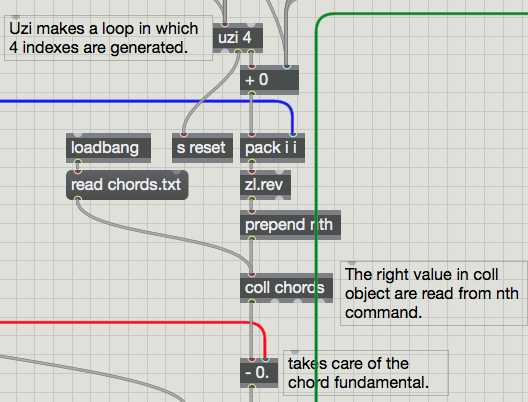
\includegraphics[width=8cm]{Figures/coll.png}
\caption{Harmonisation core stage.}
\label{coll}
\end{center}
\end{figure}
This text file is loaded immediately at the initialisation of the patcher (this is done using the \emph{loadbang} object). The file is made of rows and columns. Each row contains all the different chords that may be selected depending on the \emph{scale mode} choice. The number of rows is equal to the number of semitones that an octave interval can contain. The columns should be read in groups of 4 because we're talking about harmonisation by chords of 4 notes. When the pitch-period harmonic function is recognised, a bang is generated together with the pitch degree value. This bang triggers the \emph{uzi} process, that is to generate a specific number of indexes at the least time amount. These one, together with the pitch degree value, are packed two at a time to make 4 couples. One of these lists contains two integer values: the first refers to the momentary harmonic function of the incoming signal, the second refers to the column in which there's a chord voice it has to be extracted. As the root key and the detected pitch-period, also this voice is in pitch value. The extraction process is made by the \emph{nth} coll argument. It allows for two values, the row one first and the column one then.

Once the desired voice is selected inside the \emph{coll} object, we have to take care about the chord fundamental. For instance, if we have a $G$ note and its harmonic function is dominant, we're expecting messages like \emph{nth 7 0}, \emph{nth 7 1} and so on - for convenience, we're assuming root key is $C$ and scale mode is Major. The pitch values these messages are going to select are 2, 5, 7, 11. These are still not the correct values because we're not taking into consideration that the chord configuration is simply given assuming $C$ as fundamental, as said in \ref{recognize}. What we must do is subtract the pitch-period scale degree to each selected values. Doing this, the new pitch values will be -5, 2, 0, 4. These are the correct values we could pass to the next stage in order to calculate the ratios for pitch shifting engine. In fact, both the lists refers to the same chord: one with $C$ as fundamental, the other with $G$ - that is our case.

%3. 'Intellichord' function
\subsection{The 'Intellichord' function}
\label{intelli}
%cita provenienza Intellichord label
One of the main limitation of a so-built harmonisation is the lack of variation in chord succession standing on the same scale degrees. For instance, using the scale modes presented above there's no difference if the user plays a II - V harmonic succession or its inverted V - II. This is quite wrong, because a musician naturally tends to harmonise differently depending on what particular succession he's playing in. For that reason, he'll harmonise differently a II if he comes from a VI rather than if he comes from a IV. The modes discussed before don't allow it. Naming it, inspiration has taken from the similar function implemented in Carmine-Emanuele Cella's \emph{Revoice}. This software has been described in \ref{subsec:time}.

Here, a different harmonisation mode that tries to care for this musical aspect is shown in Figure \ref{intelli}.
\begin{figure}[htbp]
\begin{center}
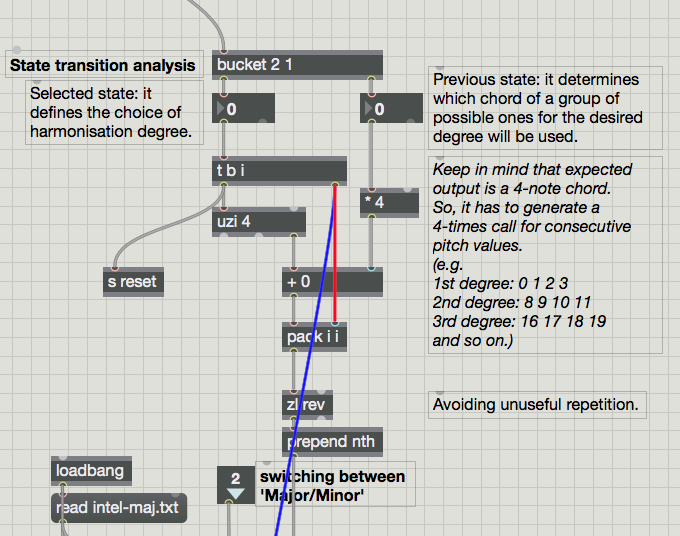
\includegraphics[width=10cm]{Figures/intelli.png}
\caption{\emph{Intellicord} engine.}
\label{intelli}
\end{center}
\end{figure}
As we could see, the process of chord selection in \emph{Intellichord} section is somewhat similar to the other one. The main differences are located before the \emph{uzi} process takes place and inside the text file that is read into the coll object. 

Let's consider the first different aspect.
The detected pitch scale degree comes into the \emph{bucket} object. This allows \emph{Intellichord} to examine every state transition between consecutive chords. In fact, before passing to a next chordal realisation the system takes memory of what scale degree it has just harmonised. Two different states (i.e. degrees) are considered at the same time. The present state defines which harmonic degree the input note is, as it's in the standard section. The previous state determines which chord of a group of possible will be used. Also this collection takes messages with the \emph{nth} argument, and for this purpose lists are created in a similar manner.

Now let's consider the text file structure:
\newline
\begin{table}[htdp]
\caption{The \emph{intelli-maj.txt} file structure.}
\begin{center}
\renewcommand{\arraystretch}{1.2}
\begin{tabular}{p{1.3cm}| p{1cm} p{1cm} p{1cm} p{1cm} p{1cm} p{1cm} p{1cm}}
\ & I & II & III & IV & V & VI & VII \\
\hline
1 & I-1 & II-1 & III-1 & IV-1 & V-1 & VI-1 & VII-1\\
2 & I-2 & II-2 & III-2 & IV-2 & V-2 & VI-2 & VII-2\\
3 & I-3 & II-3 & III-3 & IV-3 & V-3 & VI-3 & VII-3\\
4 & I-4 & II-4 & III-4 & IV-4 & V-4 & VI-4 & VII-4\\
5 & I-5 & II-5 & III-5 & IV-5 & V-5 & VI-5 & VII-5\\
6 & I-6 & II-6 & III-6 & IV-6 & V-6 & VI-6 & VII-6\\
7 & I-7 & II-7 & III-7 & IV-7 & V-7 & VI-7 & VII-7\\
\end{tabular}
\end{center}
\label{intellitable}
\end{table}
\newline
As shown in Table \ref{intellitable}, the first column indicates which scale degree we are moving from, while the first row indicates which scale degree now has to be considered. There's an implicit clockwise movement, whose final point is the cell that contains the chord that will be used for that specific succession. For instance, if the user would move from II to V, \emph{Intellichord} is going to select the chord inside the cell V-2. If the user was moving from IV to I, \emph{Intellichord} would use the chord in cell I-4. Initials inside every cell show the state transition we're talking. Roman numbers indicate the present state, arabic numbers the previous state. 

The main feature of this organisation is that there are 7 possible chords for every harmonic function the device may use, supposing all the state transitions between every scale degree are allowed. This leads to a matrix made of $7 \cdot 7 = 49$ different combinations, and so a greater dynamism in harmonising an incoming signal. Obviously, also the chord configuration in this file is given in pitch values. Differently from the \emph{chords.txt} file, here the chord fundamental is taken into account. 

\section{Interface and performance}
\label{performance}
Now, let's have a quick look at the controls provided to the user for better helping him during a performance situation.


%1. input signal control stage
\subsection{\emph{General Parameters} control stage.}
One aspect the user should notice is that the interface is well-divided into general sections. The first section presented herein, \emph{General Parameters}, contains the most important and basic controls over the entire device.
\begin{figure}[htbp]
\begin{center}
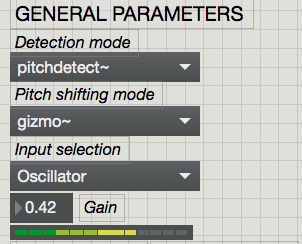
\includegraphics[width=5cm]{Figures/general.png}
\caption{\emph{General Parameters} interface section.}
\label{general}
\end{center}
\end{figure}
Here, the user can switch between several different pitch estimation algorithms. 
\newline
At the present moment, there are two pitch detection algorithms. One, pitchdetect$\sim$, is made by the Author and the Supervisor and its features are well-described in \ref{pitch}. The other, pitch$\sim$, was developed in 2001 by Tristan Jehan and is based on another MSP external, fiddle$\sim$, originally developed by Miller Puckette in fall '90s \cite{puckette1998real}.	
Moreover the user can switch between two different pitch shifting algorithms: gizmo$\sim$ and dlshift$\sim$. As the second has been discussed previously in \ref{dlshift}, \emph{gizmo} is included directly inside Max 7. This object implements a frequency-domain pitch shifting (see \ref{subsec:freq}).
\newline
The concept on which the selection has been done is to give the user the chance to choose and try at least one algorithm for each approach, both for pitch estimation and for pitch shifting. All the algorithms built and discussed in this project works in the time-based approach, instead the other belong to the frequency-domain approach.

Finally, the user is given the control over three different input signal modes: \begin{itemize}
\item \emph{External} allows for real-time performance. In fact, this choice lets the Intelligent Harmonizer take any signal coming directly from an input device, e.g. a microphone or an instrument. The input device is previously set into the Max \emph{Audio Status} window;
\item \emph{Audiofile} is the option the user has to select if he wants to harmonise some audio sample;
\item \emph{Oscillator} feeds the device algorithms with a sine oscillator, whose frequency can be manually controlled via MIDI controller or via the device itself. In fact, when choosing this option a window that shows a virtual keyboard will open. The user may change the oscillator frequency selecting the note onto this keyboard. 
\end{itemize}
Also a gain control is provided. The user can adjust the input signal amplitude looking at the level meter and finding the desired one.

%2. beyond harmonisation: delay and modulations
\subsection{Beyond shifting: \emph{delay} and \emph{modulations}.}
The following section gives some features that may help the user to achieve a better harmonisation experience. 
\newline
\begin{figure}[htbp]
\begin{center}
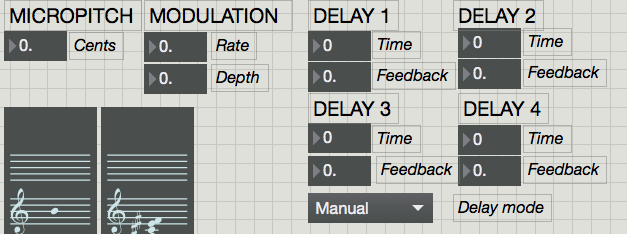
\includegraphics[width=9cm]{Figures/modulations.png}
\caption{The \emph{modulation effect} section.}
\label{mods}
\end{center}
\end{figure}
\newline
As shown in Figure \ref{mods}, the user is given two effect typologies: \emph{delay} effects and based-\emph{modulation} effects.
Delay can be used in several ways. First of all, it can replicate the character of a small vocal group in which the notes of a chord surely don't start at the same moment. It acts producing a \emph{smeared} chord attack. Every singer has his own characteristic vocal emission, and also the \emph{envelope} is involved. Moreover, the singer's own reaction time can affect the moment in which the vocal emission starts. In order to smooth the chord attack and to allow for a more natural-feel sound, each voice has its own delay with unique \emph{length} and \emph{feedback} controls. The first control is the key for achieving the effect mentioned above, and also true delay effects if the delay time overcomes small values, e.g. those in the range 20 - 80 ms. The second control produces interesting arpeggios effect \cite{lazzarini2010audio} and can also produces an interesting \emph{blurred} harmony effect. Feedback retains a small portion of the just harmonised note into the delay line, while a new harmonisation is passing through. This generates a blend between notes that belong to different chords and harmonic contexts: a sort of \emph{impressionism} in music. If we're thinking at the delay time parameter in a creative way, it's possible to realise rhythmic patterns simply providing all the delays with different and audible time settings. Finally, a \emph{historical} parameter that comes from Eventide H9 \emph{Quadravox} pitch shifting algorithm has been included. Switching this control from \emph{Manual} to \emph{Fixed}, the four delays aren't independently variable any more. In Fixed mode, the Delay 1 Time affects all the other ones in a manner that makes Delay 2 Time be longer than Delay 1, Delay 3 Time longer than Delay 2, and so on.

\emph{Modulation} provides an LFO that can be used to achieve a classic \emph{vibrato} effect. It consists of a periodic shifting that tends to simulate the natural imperfections of the vocal emission, and also the particular effect a musician can get on his instrument (for instance, by modulating a guitar string, or using the whammy bar on an electric guitar). We also can think of a vibrato as a vocal technique that comes from a spontaneous nervous tremor in the diaphragm and that can be improved and used on purpose to add expression in music. Since vibrato is typically characterised in terms of amount of pitch variation (that is, the \emph{extent} of a vibrato) and the speed at which the pitch is varied (the \emph{rate} of vibrato), the interface gives the user two independent controls: \emph{depth} and \emph{rate} \cite{cipriani2009musica}.

\emph{Micropitch} is what in Eventide's H910/H949 Harmonizer models was called \emph{Fine Control}. In particular, this control allowed for fine adjustment around Unison when the Micro mode was selected. But generally, this control affected the general pitch shifting ratio controls. Here, the concept of micropitch is quite different. The selection of the ratios, that has been described in \ref{harmonisation}, is not altered. More specifically, this is an addition to the calculated ratios. The control allows for a $\pm50$ cents adjustment and all the voices are affected in the same mode.

%3. output control stage
\subsection{Output control stage.}
\newline
\begin{figure}[htbp]
\begin{center}
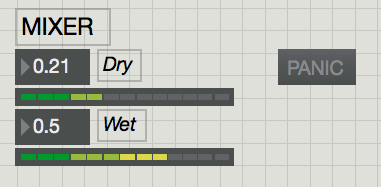
\includegraphics[width=7cm]{Figures/mixer.png}
\caption{The \emph{Mixer} section.}
\label{mixer}
\end{center}
\end{figure}
\newline
Finally, the interface gives the user the control of the level of harmonised sound (\emph{wet} parameter) and direct signal (\emph{dry} parameter). Both the parameters are given in linear amplitude, that is, they range from 0 (no sound) to 1. No gain in this stage is allowed because the user can directly act both on the input level and on each of harmonisation voices if he wants to raise the overall level.
It's also provided a useful \emph{panic} button. If pushed, it stops immediately all the DSP processes and neither input nor output signal can be heard. To restore the correct function of the device, the user has to be start again the DSP engine from the Max \emph{Audio Status} window. In order to prevent undesired sounds when DSP is turning on again, \emph{panic} makes all the input and output levels set to their minimum.

\section{Issues and future enhancements}
\label{future}
%aggiungere: pitch shifting con delay line � metodo debole. opportuno sostituire con algoritmi pi� potenti, quali ad esempio PV o PSOLA;
%aggiungere: AMDF pu� generare errori di pitch detection in casi di materiale critico; opportuno studiare implementazioni pi� robuste che limitino la possibilit� di errore;

%musical aspects improvements
Harmonisation process is a very personal one. Numerous treatises on music harmony have furnished many students different ways of harmonic realisation. There has been no definitive formalisation until now. 
As Piston wrote in \cite{piston1978harmony}:
\begin{quote}
\scriptsize{True harmonisation, then, means a consideration of the \emph{alternatives} in available chords, the reasoned selection of one of these alternatives, and the tasteful arrangement of the texture of the added pans with due regard for consistency of style. (p. 152)}
\end{quote}
Surely, the idea of harmonisation including specific musical style codified aspects is not the aim of this work. Generally, a Harmonizer has often been seen as a way of getting a quickly harmonisation and there has been not so much attention on the quality of its realisation, considering not the technical but rather the musical aspect. As shown in \ref{harmonisation}, also this device does not pay attention in the choice of arrangement and in the choice of a better alternative chord relative to the context. In fact, what our Harmonizer does is to read a table and get out the selected pitch values. If the \emph{scale mode} is changing, the selected chord will be different. But, internal to a specific harmonisation mode, there's no alternatives in available chords. This means that, for the same note, the same chord will always be selected. Moreover, there's no attention to any melodic lines as it should be in a classic four-voice writing. The concept of \emph{mutual connectibility} exposed by Piston in his own manual is not considered. In practice, most of the musical aspects and heuristics for an appropriate harmonisation are missing. This is a normal issue regarding many harmonizers, due to the fact these devices should be first very accessible to a vast range of utilisers and are affected by all the computing and technology limitations.\\
A first attempt to solve this lack of musical considerations can be seen in the development of our \emph{Intellichord} function, as shown above in \ref{intelli}. This harmonisation mode does not care about style or any arrangement taste, but focuses on the recognition of the state transitions in order to make a reasoned selection inside a range of several alternative chords. 

%1. more strategies in achieving interesting harmonisations?
\subsection{Probabilistic networks?}
In the recent time, the research focused on non-deterministic approaches and on the use of logical and mathematical assumptions in order to obtain more sophisticated harmonic realisations in a manner that can take into account a pseudo human experience. In fact, Artificial Intelligence is not able to capture the musical style of a human composer \cite{boltzmann1994}, and all his symbolic representations. This symbols make a particular rule be effectively good to describe a specific musical character, that is the \emph{style}. So, more and more diffuse is the use of probabilistic frameworks or the use of neural systems that allow to create a harmonisation system which ``\emph{learns} from examples'' \cite{allan2005harmonising} and experience. In particular, we'll provide a short description of two of these.\\
The first uses a data set of chorale harmonisations to train a Hidden Markov Model. This learning task allows to build a model of harmonic processes that can be used to compose novel harmonisations that follow particular aesthetic preferences of a wanted style, due to the clearly understanding of the basic rules of harmonisation \cite{allan2005harmonising}. The second uses neural networks both in training task and in the harmonisation process. In particular, it's been designed a learning system based on the Boltzmann Machine which allows to learn a particular harmonisation style \cite{boltzmann1994}. The same system can be used with adjustment and constraints (that is, the harmonic \emph{rules}) to harmonise music via completion.

%discussion over probabilistic networks
We can observe how the examples are focused mainly on two characteristics. First, both of the processes are non-deterministic and based on probabilistic networks. This means that there are not pre-configured tables of chords, as it's our case. The system makes a choice between different combinatoric possibilities, looking for the one that better suits the requested harmonisation. This process depends both on the nature of the melody and on the stochastic nature of the models involved (Boltzmann distribution, or Markov Model for instance). We can speak in some way of a real harmonic \emph{synthesis}. This also makes the system perform different results even if the melody is the same. Secondly, both of the examples allows for machine-learning music harmonisation systems. Given the advance in machine learning, it's desirable to apply its techniques to music harmony so to build a system that learns to harmonise and to distinguish between different musical styles. So, the great advantage of this networks is that they are capable of learning internal representations and are also able to solve difficult combinatoric problems. Doing so, the chord construction and its displacement over four voice is truly a real-time task. 

Perhaps, one issue about Boltzmann Machine is that it could stop learning correctly. Learning in general Boltzmann Machine is quite impractical, so it could be made useful to properly constrain the connectivity. This means to insert external constraints in order to let the process efficient enough, whereas the Hidden Markov Model example learns its harmonisation constraints directly from training data. These external constraints are vital to the success of the Boltzmann Machine harmonisation system. Moreover, neural networks are less compute-intensive, but these harmonisation systems retain a pre-programmed knowledge base \cite{allan2005harmonising}. They take a large set of rules written by a human, and so could penalise undesirable combinations of notes so that they can be filtered out. Instead, Markov models don't need predetermined tune or implicit control knowledge.

In conclusion, several system have applied probabilistic networks to harmonisation. Using these kind of system allows to perform more efficient inference to generate new harmonisations. It's also possible to let the system itself learn from adequate examples provided by an external user. In this manner, learning processes and techniques takes importance as much as the harmonisation process itself. The choice of right notes to complete a specific chord and the choice of which harmonic formulae the system should use in a specific content should be made by stochastic models. They allow for non-repetitive patterns, even if the harmonised material doesn't change. In a musical view, these characteristics would be a truly improvement for this kind of device. They perhaps require lots of non-musical knowledge, as most of the concepts come from mathematics and statistic. Further information about HMM-based harmonisation model can be found in \cite{ueda2010hmm}, as in \cite{paiement2006probabilistic} different representation for musical chords that are presented. 

\section{Conclusion}
\label{ending}
In this chapter, we focused mainly on the musical aspects of this project.
First, we described the process that lets this Harmonizer be \emph{intelligent}, that is to recognise every pitch-period harmonic function so to give it a specific scale degree, depending on the selected root key. Then, we described the different typologies of harmonisation that the device provides the user, and how the chords are selected. A more accurate harmonisation model, \emph{Intellichord}, is also shown. Later in the chapter, the user interface was shown in details. All its section were described, and also all the effects and controls. Finally, it's been provided a briefly discussion about possible enhancements so to realise a more complete, ready-to-use and sophisticate device. 

At the end of this paper, we can observe that all this work is undoubtedly acceptable. Nevertheless, several improvements and a change for the better are recommended. In particular, the realm of harmonisation system should be enhanced to give it a more flexible behaviour.
The Author wishes for a possible work of revision and improvement during the successive years.







%----------------------------------------------------------------------------------------
%	THESIS CONTENT - APPENDICES
%----------------------------------------------------------------------------------------

\addtocontents{toc}{\vspace{2em}} % Add a gap in the Contents, for aesthetics

\appendix % Cue to tell LaTeX that the following 'chapters' are Appendices

% Include the appendices of the thesis as separate files from the Appendices folder
% Uncomment the lines as you write the Appendices

% Appendix A

\chapter{Source code} % Main appendix title

\label{AppendixA} % For referencing this appendix elsewhere, use \ref{AppendixA}

\lhead{Appendix A. \emph{Source code}} % This is for the header on each page - perhaps a shortened title

Here are presented, for documentation, the codes of the two realised algorithms, pitchdetect$\sim$ and dlshift$\sim$.
Both of them are included in the header file \emph{dsp.h} and are the core of their own MSP externals.

All this codes are written using C++ programming language.
\newline
\newline
\newline
\section{AMDF-based pitch detection}
\lstinputlisting[caption=AMDF-based pitch detection]{Code/amdf.cpp}
\null\vfill
\section{Delay-line base pitch shifting}
\lstinputlisting[caption=Delay-line base pitch transposition]{Code/dlshift.cpp}

% Appendix A

\chapter{MSP external code} % Main appendix title

\label{AppendixB} % For referencing this appendix elsewhere, use \ref{AppendixA}

\lhead{Appendix B. \emph{MSP external code}} % This is for the header on each page - perhaps a shortened title

Here, the main methods of the two externals built in Xcode 6, labelled \emph{perform}, are presented.
They are excerpts of a longer codes that include all the information about MSP external construction, initialisation and all the methods with which the user can set the object and modify its behaviour. 
\newline
Generally, everyone of these codes contains a section relative to the class making. In fact, each externals has an internal class that specifies all the member variables used by its own functions and all the methods. For simplicity, the DSP class method is always called \emph{perform}. It's a void function that is called when the audio turns on in Max. 
\newline
Finally, every class contains two function named as the class itself. One is the initialisation function, the so-called \emph{constructor}. The other is the \emph{destructor}, that is the function acting when the external is removed into the Max patcher. The purpose of this function is to free the memory previously occupied by interal buffers. 

All this codes are written using C++ programming language.
\newline
\newline
\newline
\section{Pitchdetect$\sim$}
\label{pitchcode}
\lstinputlisting[caption=The pitchdetect$\sim$ \emph{perform} function]{Code/pitchdetect.cpp}
\section{Dlshift$\sim$}
\label{shiftcode}
\lstinputlisting[caption=The dlshift$\sim$ \emph{perform} function]{Code/dlshifter.cpp}


\addtocontents{toc}{\vspace{2em}} % Add a gap in the Contents, for aesthetics

\backmatter

%----------------------------------------------------------------------------------------
%	BIBLIOGRAPHY
%----------------------------------------------------------------------------------------

\label{Bibliography}

\lhead{\emph{Bibliography}} % Change the page header to say "Bibliography"

\bibliographystyle{unsrtnat} % Use the "unsrtnat" BibTeX style for formatting the Bibliography

\bibliography{Bibliography} % The references (bibliography) information are stored in the file named "Bibliography.bib"

\nocite{*}

\clearpage


%----------------------------------------------------------------------------------------
%	ABSTRACT (ITA)
%----------------------------------------------------------------------------------------

\abstract{\addtocontents{toc}{\vspace{1em}} % Add a gap in the Contents, for aesthetics

Viene definita \emph{armonia} l'organizzazione delle altezze di un suono polifonico all'interno di un intervallo temporale. L'altezza di un suono armonico (inteso come suono scomponibile nelle sue componenti tramite la serie di Fourier) pu\`o essere trasportato. Questo avviene tramite la tecnica del \emph{pitch shifting}, ovvero la modifica del contenuto frequenziale di un segnale ottenuta moltiplicandolo per una \emph{ratio} specifica. In generale, un suono viene \emph{armonizzato} se ad esso vengono aggiunte differenti versioni trasportate al fine di generare un accordo. Si intende armonizzazione intelligente, o \emph{smart harmony}, un processo che tiene conto sia del contesto armonico sia del fondamentale del segnale. A tal scopo, \`e necessario l'utilizzo di un algoritmo per la stima della frequenza fondamentale del segnale.
}

\end{document}  